%!TEX program = xelatex
% 完整编译方法 1 pdflatex -> bibtex -> pdflatex -> pdflatex
% 完整编译方法 2: xelatex -> bibtex -> xelatex -> xelatex
\documentclass[lang=cn,11pt]{elegantpaper}
\usepackage{latexsym}

\title{感应式无线电能传输系统的传输距离极限}
\author{\href{https://gitee.com/lonelybag/personal-doc/}{Lonelybag}}

% \institute{\href{https://elegantlatex.org/}{Elegant\LaTeX{} 项目组}}

% 不需要版本信息,直接注释即可
\version{0.1}
% 不需要时间信息的话,需要把 \today 删除。
\date{\today}

\begin{document}
\maketitle

\begin{abstract}
  基于电磁场理论推导磁偶极子和电偶极子的近场传输距离极限。
  \begin{itemize}
    \item 目的:探究感应式无线电能传输的传输距离极限
    \item 研究方法:基于电磁场理论推导磁偶极子和电偶极子的电磁场表达式并绘制函数图像,总结近场电磁场空间时间分布规律
    \item 结论:
    \begin{itemize}
      \item 空间特性:近场范围是$\frac{\lambda}{2\pi}$
      \item 时间特性:近场中,电磁场呈现驻波特性
    \end{itemize}
  \end{itemize}

\keywords{电磁场,磁偶极子,电偶极子,近场}
\end{abstract}

\section{电偶极子}
\begin{itemize}
  \item $\beta=\omega\sqrt{LC}=\omega\sqrt{\mu\epsilon}(rad/m)$ - 相移
  \item $v=\frac{1}{\sqrt{LC}}=\frac{1}{\sqrt{\mu \epsilon}}$ - 波速
  \item $\eta=\sqrt{\frac{L}{C}}=\sqrt{\frac{\mu}{\epsilon}}$ - 特征阻抗
  \item $\widetilde{I}$ - 电流幅值
\end{itemize}
\subsection{理论推导}
\begin{figure}[ht]
  \centering
  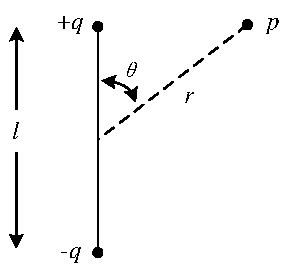
\includegraphics[width=0.3\linewidth]{figure//Hertzian_Dipole.pdf}
  \vspace{-0.3cm}
  \caption{电偶极子}\label{fig:Hertazian_Dipole}
\end{figure}
首先推导磁场
\begin{equation}
  \begin{aligned}
    \vec{H} &= \frac{1}{\mu}\left[\nabla\times \vec{A} \right] \\
            & = \frac{j\beta \widetilde{I}l}{4\pi r}\left(1 + \frac{1}{j\beta r}\right)sin \theta {} e^{-j\beta r} \vec{a_{\phi}}
\end{aligned}
\end{equation}
可以看出,磁场的图像是一簇水平曲线。然后推导电场
\begin{equation}
  \begin{aligned}
    \vec{E} &= \frac{1}{j\omega \epsilon}\left[\nabla \times \vec{H}\right] \\
    &= \frac{\eta \widetilde{I}l}{2\pi r^2}\left(1 + \frac{1}{j\beta r} \right)cos\theta e^{-j\beta r}\vec{a_r}+\frac{j\widetilde{l\eta \beta}}{4\pi r}\left(1+\frac{1}{j\beta r} - \frac{1}{{\beta}^2r^2}\right)sin\theta e^{-j\beta r}\vec{a_{\theta}}
  \end{aligned}
\end{equation}
可以看出,电场是垂直于平面的一簇曲线。
\subsection{近场}
定义$\beta r \ll 1$的区域为近场区(near-zone fields)\footnote{也即,近场区域内,空间电磁场的相位差远远小于1 $rad$。}。由此可以得到下列近似
\begin{equation}
  \left\{\begin{aligned}
    & e^{-j\beta r}\rightarrow 1 \\
    & 1 + \frac{1}{j\beta r} \rightarrow \frac{1}{j\beta r} \\
    & 1 + \frac{1}{j\beta r} - \frac{1}{{\beta}^2 r^2} \rightarrow \frac{1}{j\beta r} - \frac{1}{{\beta}^2 r^2}
  \end{aligned}\right.
\end{equation}

因此,可以得到近场磁场方程
\begin{equation}
  \begin{aligned}
    \vec{H} &= \frac{j\beta \widetilde{I}l}{4\pi r}\left(1 + \frac{1}{j\beta r}\right)sin \theta {} e^{-j\beta r} \vec{a_{\phi}} \\
    &\xrightarrow[1 + \frac{1}{j\beta r}\rightarrow \frac{1}{j\beta r}]{e^{j\beta r}\rightarrow 1} \frac{\widetilde{I}l}{4\pi r^2}sin \theta \vec{a_{\phi}} 
  \end{aligned}
\end{equation}
类似的,也可以得到近场电场方程
\begin{equation}
  \begin{aligned}
    \vec{E} &= \frac{1}{j\omega \epsilon}\left[\nabla \times \vec{H}\right] \\
    &= \frac{\eta \widetilde{I}l}{2\pi r^2}\left(1 + \frac{1}{j\beta r} \right)cos\theta e^{-j\beta r}\vec{a_r}+\frac{j\widetilde{l\eta \beta}}{4\pi r}\left(1+\frac{1}{j\beta r} - \frac{1}{{\beta}^2r^2}\right)sin\theta e^{-j\beta r}\vec{a_{\theta}} \\
    &\xrightarrow[1 + \frac{1}{j\beta r} -\frac{1}{{\beta}^2r^r}\rightarrow \frac{1}{j\beta r}-\frac{1}{{\beta}^2r^r}]{e^{j\beta r}\rightarrow 1} \\
    & \frac{\eta \widetilde{I}l}{4\pi r^2}\left(1+\frac{1}{j\beta r}\right)2cos\theta e^{-j\beta r}\vec{a_r}+\frac{j\widetilde{I}l\eta \beta}{4\pi r}\left(\frac{1}{j\beta r}\right)\left( 1+\frac{1}{j\beta r}\right)sin\theta e^{-j\beta r}\vec{a_{\theta}}\\
    &= \frac{\eta \widetilde{I}l}{4\pi r^2}\left(1+\frac{1}{j\beta r}\right)2cos\theta \vec{a_r} +\frac{\widetilde{I}l\eta}{4\pi r^2}\left( 1+\frac{1}{j\beta r}\right)sin\theta \vec{a_{\theta}} \\
    &= \frac{\eta \widetilde{I}l}{4\pi r^2}\left(1+\frac{1}{j\beta r}\right)\left(2cos\theta \vec{a_r} + sin\theta \vec{a_{\theta}}\right)
  \end{aligned}
\end{equation}

\subsection{仿真}

\section{磁偶极子}
\begin{itemize}
  \item $\widetilde{I}$ - 电流幅值
  \item $a$ - 线圈半径
  \item $r$ - 距离
\end{itemize}
\subsection{理论推导}
\begin{figure}[ht]
  \centering
  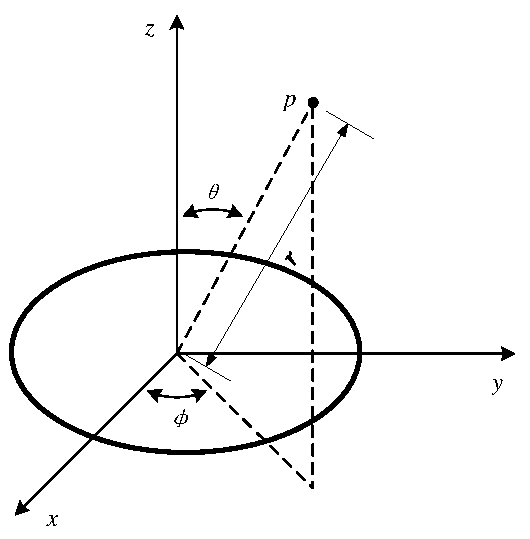
\includegraphics[width=0.3\linewidth]{figure//Magnetic_Dipole.pdf}
  \vspace{-0.3cm}
  \caption{磁偶偶极子}\label{fig:Magnetic_Dipole}
\end{figure}
首先推导磁场
\begin{equation}
  \begin{aligned}
    \vec{E} = -j\frac{\omega \mu (\pi a^2)\widetilde{I}\beta}{4\pi r}\left(1+\frac{1}{j\beta r}\right)sin\theta e^{-j\beta r}\vec{a_{\phi}}
\end{aligned}
\end{equation}
然后推导磁场
\begin{equation}
  \begin{aligned}
    \vec{H} = j\frac{\omega \mu (\pi a^2)\widetilde{I}}{2\pi r^2\eta}\left(1+\frac{1}{j\beta r}\right)cos\theta e^{-j\beta r}\vec{a_r} + j\frac{\omega (\pi a^2)\widetilde{I}\beta}{4\pi r \eta}\left(1+\frac{1}{j\beta r} - \frac{1}{{\beta}^2 r^2}\right)sin\theta e^{-j\beta r}\vec{a_{\theta}}
\end{aligned}
\end{equation}

\subsection{近场}
定义$\beta r \ll 1$的区域为近场区(near-zone fields)。由此可以得到
\begin{equation}
  \begin{aligned}
    \beta &= \omega\sqrt{\mu \epsilon} = 2\pi f \sqrt{\mu \epsilon} \xrightarrow{v = \frac{1}{\sqrt{\mu \epsilon}}} \beta = \frac{2\pi}{\lambda} \\
    &\xrightarrow{r\ll \frac{1}{\beta}} r\ll \frac{\lambda}{2\pi}
  \end{aligned}
\end{equation}
因此可以认为,近场区为距离偶极子$\frac{\lambda}{2\pi}$以内的区域。

\nocite{*}

\bibliography{ref}

\end{document}
